\documentclass[12pt, a4paper]{article}

% --- Packages ---
\usepackage[utf8]{inputenc} % Allow input of international characters
\usepackage[T1]{fontenc}    % Output font encoding for international characters
\usepackage{geometry}       % For page layout and margins
\usepackage{amsmath}        % For advanced math typesetting
\usepackage{graphicx}       % For including images
\usepackage{hyperref}       % For hyperlinks in the PDF
\usepackage{xcolor}         % For colored text
\usepackage{tikz}           % For diagrams
\usetikzlibrary{positioning, shapes.geometric, arrows.meta, fit, backgrounds, calc}
\usepackage{pifont}         % For checkmark and X symbols

% --- TikZ Layer Setup ---
\pgfdeclarelayer{vmlayer}
\pgfdeclarelayer{containerlayer}
\pgfsetlayers{vmlayer,containerlayer,main}

% --- Diagram Colors ---
\definecolor{vmcolor}{RGB}{220,220,220}
\definecolor{bsuicolor}{RGB}{173,216,230}
\definecolor{bsuiborder}{RGB}{70,130,180}
\definecolor{erobscolor}{RGB}{144,238,144}
\definecolor{erobsborder}{RGB}{60,139,60}
\definecolor{componentbg}{RGB}{255,255,255}
\definecolor{robotcolor}{RGB}{255,200,124}
\definecolor{arrowcolor}{RGB}{70,130,180}
\definecolor{servercolor}{RGB}{200,180,230}
\definecolor{cameracolor}{RGB}{180,220,255}
\usepackage{booktabs}       % For professional tables
\usepackage{array}          % For column formatting
\usepackage{makecell}       % For line breaks in cells
\usepackage{float}          % For [H] float placement

% --- Custom Commands ---
\newcommand{\yes}{\textcolor{green!60!black}{\ding{51}}}
\newcommand{\no}{\textcolor{red!70!black}{\ding{55}}}
\newcommand{\maybe}{\textcolor{orange!80!black}{$\sim$}}
\newcommand{\tbd}{--}

% --- Page Layout ---
\geometry{margin=1in}

% --- Document Metadata ---
\title{Current Blockers}
\author{Your Name}
\date{\today}

\begin{document}

\maketitle

\section{Drylab VM}
Drylab VM is required for development / testing before deploying at the beamline. Currently all development is being done locally on a laptop and VM based implementation is only being done at the beamline during maintenance/shutdown. A working Drylab VM will allow a robust implementation with less time spent debugging issues when at the beamline.
\begin{enumerate}
    \item VM is @ 10.69.26.42 / lob4-ros1
    \item Robot is @ 10.69.26.41
\end{enumerate}
\subsection{Socket Communication issue}

% Socket Communication Diagram
\begin{figure}[H]
\centering
\begin{tikzpicture}[
    node distance=5cm,
    arrow/.style={-{Stealth[length=3mm, width=2mm]}, line width=1.5pt},
]
    % === VM Icon (Computer/Server) ===
    \begin{scope}[local bounding box=vmicon]
        % Monitor
        \draw[thick, fill=blue!20] (-0.6,-0.1) rectangle (0.6,0.7);
        \draw[thick, fill=blue!40] (-0.5,0) rectangle (0.5,0.6);
        % Stand
        \draw[thick, fill=gray!40] (-0.15,-0.1) rectangle (0.15,-0.3);
        \draw[thick, fill=gray!40] (-0.3,-0.3) rectangle (0.3,-0.4);
    \end{scope}
    \node[below=0.1cm of vmicon, font=\bfseries] (vmlabel) {VM};
    \node[below=0pt of vmlabel, font=\footnotesize\ttfamily] (vmip) {10.69.26.42};

    % === UR Robot (Actual Image) ===
    \node[inner sep=0pt] (roboticon) at (5.5,0.15)
        {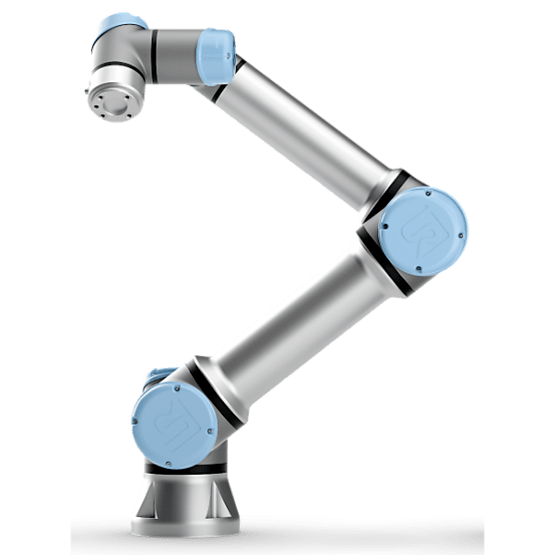
\includegraphics[width=2cm]{images/ur5e.png}};
    \node[below=0.1cm of roboticon, font=\bfseries] (robotlabel) {UR Robot};
    \node[below=0pt of robotlabel, font=\footnotesize\ttfamily] (robotip) {10.69.26.41};

    % === Arrows ===
    % VM -> Robot (works)
    \draw[arrow, green!60!black]
        (0.8,0.6) -- (4.4,0.6)
        node[midway, above=2pt, green!60!black, font=\Large] {\ding{51}};

    % Robot -> VM (fails)
    \draw[arrow, red!70!black]
        (4.4,-0.1) -- (0.8,-0.1)
        node[midway, below=2pt, red!70!black, font=\Large] {\ding{55}};

\end{tikzpicture}
\caption{VM can connect to robot, but robot cannot communicate back to VM.}
\label{fig:socket-comm}
\end{figure}

\begin{enumerate}
  \item Robot successfully connects with the VM and connection is verified by ping 
  \item UR Cap (UR Software plugin to allow controlling the robot from PC/laptop) requires ports 50001-50004 for communication.(currently fails)
  \item Verified the socket communication issue by running a test socket server / client between laptop and VM (no robot)
  \begin{enumerate}
    \item Laptop as server , VM as client - works \textcolor{green!60!black}{\ding{51}}
    \item Laptop as client and VM as server - fails \textcolor{red!70!black}{\ding{55}}
  \end{enumerate}
  \item  Possible solution is to modify $/etc/nftables/main.nft$ to open required ports in the VM.
  \item Communication works without issues at beamline VM.
\end{enumerate}

\subsection{Cameras}
\begin{enumerate}
  \item Zivid Camera requires an IP at drylab - preferably on the same subnet as the robot.
  \item ZED cameras require setting up the Digi USB anywhere (USB $\rightarrow$ Ethernet) as well as IP. 
  \item Require GPU resource 
\end{enumerate}

\section{Beamline VM}
\subsection{Cameras}
\begin{enumerate}
  \item Zivid Camera is not discoverable from VM (Camera is on CAM subnet , VM is on INST subnet?)
  \begin{enumerate}
    \item either reconfigure the VM to have additional interface with CAM subnet
    \item or configure the camera in the same subnet as the robot (as an extension of the robot)
  \end{enumerate}
  \item ZED cameras require Digi Anywhere USB to be setup.
  \item All cameras require GPU compute which is currently unavailable.
\end{enumerate}
\subsection{Bluesky/EPICS}
\begin{enumerate}
  \item Bluesky on VM cannot communicate with EPICS/other beamline hardware.
\end{enumerate}


\section{GPU Requirements}

Both Zivid and ZED camera systems require dedicated NVIDIA GPU resources for point cloud processing. This is a hard requirement; the cameras cannot function without GPU acceleration.

\begin{table}[H]
\centering
\small
\renewcommand{\arraystretch}{1.3}
\resizebox{\textwidth}{!}{%
\begin{tabular}{@{}lccc@{}}
\toprule
\textbf{Requirement} & \textbf{Zivid 2+} & \textbf{ZED 2i} & \makecell{\textbf{Current Setup}\\\footnotesize(1$\times$ Zivid + 2$\times$ ZED 2i)} \\
\midrule
Min. GPU Memory (VRAM) & 3 GB & 6+ GB & \textbf{12+ GB} \\
Min. GPU             & GTX 1060+ & RTX 20-series+ & \textbf{RTX 40-series+} \\
\midrule
Interface            & 10GbE & USB 3.0 & 10GbE + 2$\times$ USB 3.0 \\
Min. RAM             & 16 GB & 8 GB & 32 GB \\
\midrule
OS Support           & Ubuntu 22.04+ & Ubuntu 22.04+ & Ubuntu 22.04 \\
\bottomrule
\end{tabular}%
}
\caption{GPU and system requirements comparison: Zivid vs ZED 2i cameras.}
\label{tab:gpu-comparison}
\end{table}

\noindent\textbf{Note:} Data center GPUs (NVIDIA H100, A100, etc.) are not officially supported by either Zivid or ZED SDKs.

\noindent\textbf{References:}
\begin{itemize}
    \item Zivid: \url{https://support.zivid.com/en/latest/getting-started/software-installation/gpu/gpu-requirements.html}
    \item ZED 2i: \url{https://www.stereolabs.com/docs/development/zed-sdk/specifications}
\end{itemize}

\subsection{Zivid Capture Time Benchmarks}
The figure below shows capture times for different GPU configurations with Manufacturing presets on Zivid 2+R.

\begin{figure}[H]
\centering
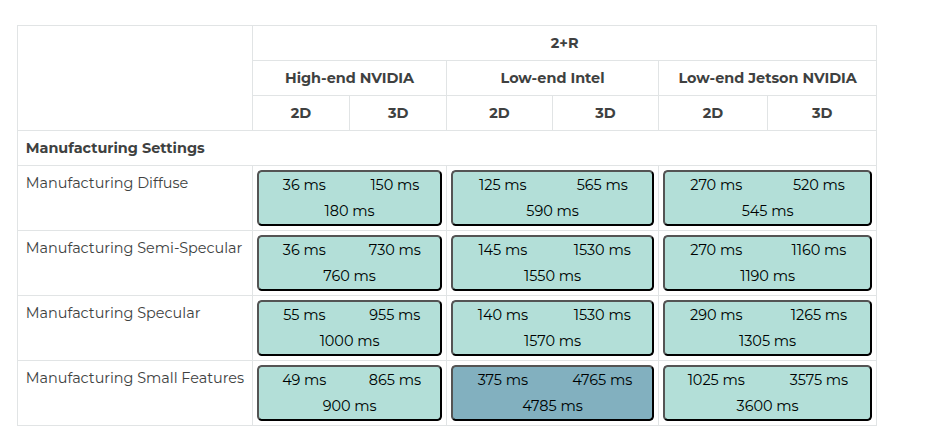
\includegraphics[width=0.9\textwidth]{images/zivid_benchmark.png}
\caption{Zivid 2+R capture times (ms) for Manufacturing presets across GPU configurations.}
\label{fig:zivid-benchmark}
\end{figure}

\section{Deployment Comparison}

\begin{table}[H]
\centering
\small
\renewcommand{\arraystretch}{1.4}
\begin{tabular}{@{}l|cccccc@{}}
\toprule
\textbf{Feature} &
\makecell{\textbf{PDF VM}\\\footnotesize(Phil)} &
\makecell{\textbf{CMS VM}\\\footnotesize(Current)} &
\makecell{\textbf{VM +}\\\textbf{GPU}} &
\makecell{\textbf{Ubuntu}\\\textbf{Workstation}} &
\makecell{\textbf{Laptop}} &
\makecell{\textbf{Jetson}} \\
\midrule
Bluesky/EPICS Access    & \yes & \no  & \yes & \yes & \no &\maybe \\
GPU Available           & \no  & \no  & \yes & \yes & \yes \\
Camera Integration      & physical server & \no  & \tbd & \yes & \yes \\

% Add more rows below as needed
% Example row:
% Feature Name          & \yes & \no  & \maybe & \tbd & \yes \\
\bottomrule
\end{tabular}
\caption{Comparison of deployment options for EROBS system.}
\label{tab:deployment-comparison}
\end{table}

\noindent
\textbf{Legend:} \yes\ = Available/Working \quad \no\ = Not Available/Failing \quad \maybe\ = Partial/Limited \quad \tbd\ = To Be Determined

\section{EROBS Deployment Architecture}
\subsection{PDF Beamline implmentation by Phil}
\begin{enumerate}
    \item Two Docker containers - one for Bluesky (bsui) and one for ROS2 (erobs)
    \item Only supports pick and place actions with predefined joint angles
    \item Camera - Azure Kinect DK connected via USB to a physical server (System 76 Meerkat)
\end{enumerate}
\begin{figure}[H]
\centering
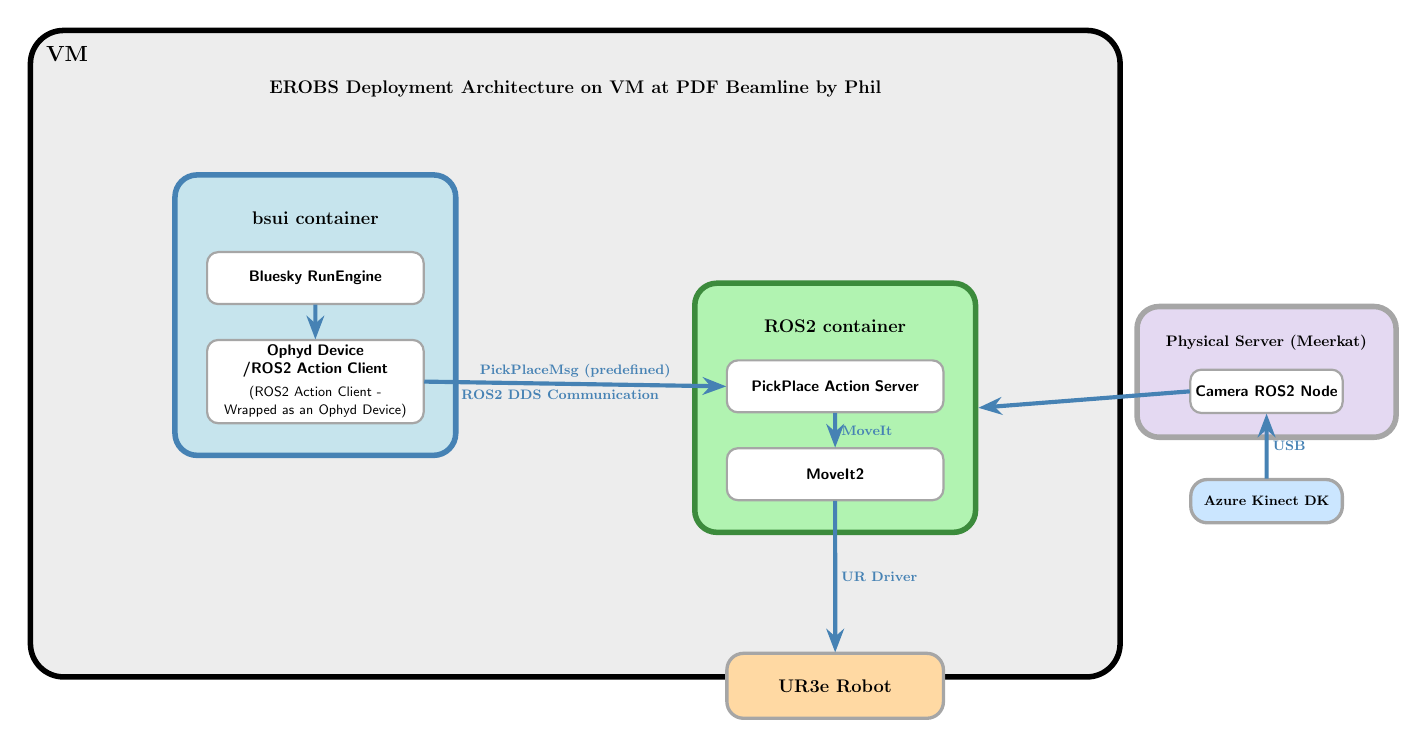
\begin{tikzpicture}[
    scale=0.55,
    transform shape,
    node distance=1.2cm,
    font=\sffamily,
    arrow/.style={-{Stealth[length=3mm]}, line width=1.5pt, color=arrowcolor},
    componentbox/.style={
        rectangle,
        rounded corners=4pt,
        minimum width=5cm,
        minimum height=1.2cm,
        text centered,
        text width=4.5cm,
        draw=gray!70,
        thick,
        fill=componentbg
    }
]

% Title
\node (title) [font=\large\bfseries] {EROBS Deployment Architecture on VM at PDF Beamline by Phil};

%% LEFT SIDE - bsui container %%
\node (bsui_title) [below=2.4cm of title, xshift=-6cm, font=\large\bfseries] {bsui container};

\node (runengine) [componentbox, below=0.5cm of bsui_title] {
    \textbf{Bluesky RunEngine}
};

\node (ophyd) [componentbox, below=0.8cm of runengine] {
    \textbf{Ophyd Device /ROS2 Action Client}\\[0.1cm]
    {\small (ROS2 Action Client - Wrapped as an Ophyd Device)}
};

%% RIGHT SIDE - ROS2 container %%
\node (erobs_title) [below=4.9cm of title, xshift=6cm, font=\large\bfseries] {ROS2 container};

\node (action_servers) [componentbox, below=0.5cm of erobs_title] {
    \textbf{PickPlace Action Server}
};

\node (moveit) [componentbox, below=0.8cm of action_servers] {
    \textbf{MoveIt2}
};

%% ROBOT (outside VM) %%
\node (robot) [
    below=3.5cm of moveit,
    rectangle,
    rounded corners=6pt,
    minimum width=5cm,
    minimum height=1.5cm,
    text centered,
    draw=gray!70,
    very thick,
    fill=robotcolor!70,
    font=\large\bfseries
] {UR3e Robot};

%% PHYSICAL SERVER (outside VM, right side) %%
\node (server_title) [
    right=5cm of action_servers,
    yshift=1cm,
    font=\bfseries
] {Physical Server (Meerkat)};

\node (camera_node) [
    below=0.3cm of server_title,
    rectangle,
    rounded corners=4pt,
    minimum width=3.5cm,
    minimum height=1cm,
    text centered,
    draw=gray!70,
    thick,
    fill=componentbg
] {\textbf{Camera ROS2 Node}};

%% CAMERA HARDWARE (below server) %%
\node (camera) [
    below=1.5cm of camera_node,
    rectangle,
    rounded corners=6pt,
    minimum width=3.5cm,
    minimum height=1cm,
    text centered,
    draw=gray!70,
    very thick,
    fill=cameracolor!70,
    font=\bfseries\small
] {Azure Kinect DK};

%% CONTAINER LAYER - Draw colored container boxes %%
\begin{pgfonlayer}{containerlayer}
    \node (bsui_container) [
        rectangle,
        rounded corners=8pt,
        fill=bsuicolor!70,
        draw=bsuiborder,
        line width=2pt,
        fit=(bsui_title)(runengine)(ophyd),
        inner sep=0.4cm
    ] {};

    \node (erobs_container) [
        rectangle,
        rounded corners=8pt,
        fill=erobscolor!70,
        draw=erobsborder,
        line width=2pt,
        fit=(erobs_title)(action_servers)(moveit),
        inner sep=0.4cm
    ] {};

    %% Server container box %%
    \node (server_box) [
        rectangle,
        rounded corners=8pt,
        fill=servercolor!50,
        draw=gray!70,
        line width=2pt,
        fit=(server_title)(camera_node),
        inner sep=0.3cm
    ] {};
\end{pgfonlayer}

%% VM LAYER - Draw VM box (deepest) %%
\begin{pgfonlayer}{vmlayer}
    \node (vm_box) [
        rectangle,
        rounded corners=12pt,
        fill=vmcolor!50,
        draw=black,
        line width=2pt,
        fit=(bsui_container)(erobs_container),
        inner sep=1.8cm
    ] {};
\end{pgfonlayer}

%% VM Label %%
\node [anchor=north west, font=\Large\bfseries, xshift=0.3cm, yshift=-0.3cm] at (vm_box.north west) {VM};

%% ARROWS %%
\draw [arrow] (runengine) -- (ophyd);

\draw [arrow] (ophyd.east) --
    node[pos=0.5, above, font=\small\bfseries] {PickPlaceMsg (predefined)}
    node[pos=0.45, below, font=\small\bfseries] {ROS2 DDS Communication}
    (action_servers.west);
\draw [arrow] (action_servers) --
    node[pos=0.5, right, font=\small\bfseries] {MoveIt}
    (moveit);

\draw [arrow] (moveit.south) --
    node[pos=0.5, right, font=\small\bfseries] {UR Driver}
    (robot.north);

%% Camera/Server arrows %%
\draw [arrow] (camera.north) --
    node[pos=0.5, right, font=\small\bfseries] {USB}
    (camera_node.south);

\draw [arrow] (camera_node.west) --
    (erobs_container.east);

\end{tikzpicture}
\caption{EROBS deployment architecture showing the two-container setup on VM at PDF beamline.}
\label{fig:erobs-architecture}
\end{figure}

\subsection{CMS Beamline Implementation on a VM}
\begin{enumerate}
    \item Two Docker containers - one for Bluesky (bsui) and one for ROS2 (erobs-common-img)
    \item Full MTC orchestrator with multiple action servers (move\_to, pick\_place, vision, etc.)
    \item JSON-based task interface for flexible experiment orchestration
\end{enumerate}

\begin{figure}[H]
\centering
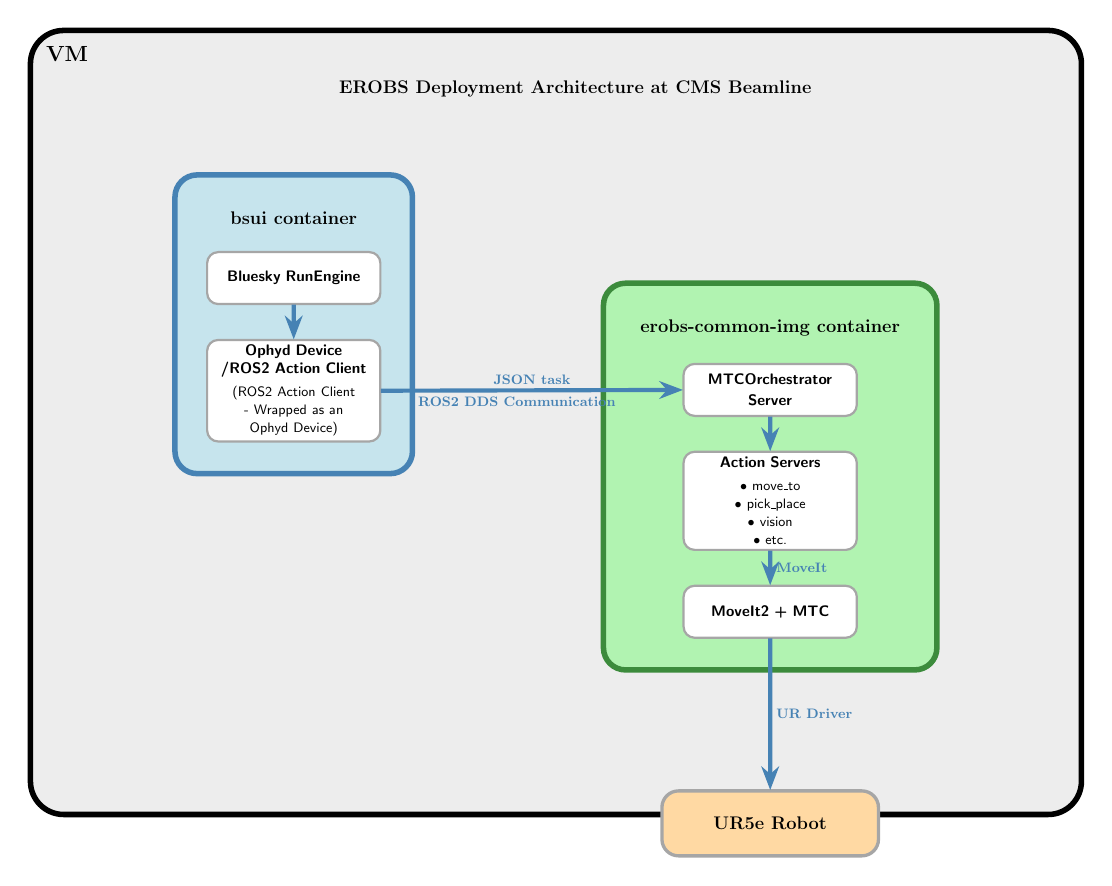
\begin{tikzpicture}[
    scale=0.55,
    transform shape,
    node distance=1.2cm,
    font=\sffamily,
    arrow/.style={-{Stealth[length=3mm]}, line width=1.5pt, color=arrowcolor},
    componentbox/.style={
        rectangle,
        rounded corners=4pt,
        minimum width=4cm,
        minimum height=1.2cm,
        text centered,
        text width=3.6cm,
        draw=gray!70,
        thick,
        fill=componentbg
    }
]

% Title
\node (title) [font=\large\bfseries] {EROBS Deployment Architecture at CMS Beamline};

%% LEFT SIDE - bsui container %%
\node (bsui_title) [below=2.4cm of title, xshift=-6.5cm, font=\large\bfseries] {bsui container};

\node (runengine) [componentbox, below=0.5cm of bsui_title] {
    \textbf{Bluesky RunEngine}
};

\node (ophyd) [componentbox, below=0.8cm of runengine] {
    \textbf{Ophyd Device /ROS2 Action Client}\\[0.1cm]
    {\small (ROS2 Action Client - Wrapped as an Ophyd Device)}
};

%% RIGHT SIDE - erobs-common-img container %%
\node (erobs_title) [below=4.9cm of title, xshift=4.5cm, font=\large\bfseries] {erobs-common-img container};

\node (orchestrator) [componentbox, below=0.5cm of erobs_title] {
    \textbf{MTCOrchestrator}\\[0.05cm]
    \textbf{Server}
};

\node (action_servers) [componentbox, below=0.8cm of orchestrator, minimum height=2.2cm] {
    \textbf{Action Servers}\\[0.1cm]
    {\small $\bullet$ move\_to}\\
    {\small $\bullet$ pick\_place}\\
    {\small $\bullet$ vision}\\
    {\small $\bullet$ etc.}
};

\node (moveit) [componentbox, below=0.8cm of action_servers] {
    \textbf{MoveIt2 + MTC}
};

%% ROBOT (outside VM) %%
\node (robot) [
    below=3.5cm of moveit,
    rectangle,
    rounded corners=6pt,
    minimum width=5cm,
    minimum height=1.5cm,
    text centered,
    draw=gray!70,
    very thick,
    fill=robotcolor!70,
    font=\large\bfseries
] {UR5e Robot};

%% CONTAINER LAYER - Draw colored container boxes %%
\begin{pgfonlayer}{containerlayer}
    \node (bsui_container) [
        rectangle,
        rounded corners=8pt,
        fill=bsuicolor!70,
        draw=bsuiborder,
        line width=2pt,
        fit=(bsui_title)(runengine)(ophyd),
        inner sep=0.4cm
    ] {};

    \node (erobs_container) [
        rectangle,
        rounded corners=8pt,
        fill=erobscolor!70,
        draw=erobsborder,
        line width=2pt,
        fit=(erobs_title)(orchestrator)(action_servers)(moveit),
        inner sep=0.4cm
    ] {};
\end{pgfonlayer}

%% VM LAYER - Draw VM box (deepest) %%
\begin{pgfonlayer}{vmlayer}
    \node (vm_box) [
        rectangle,
        rounded corners=12pt,
        fill=vmcolor!50,
        draw=black,
        line width=2pt,
        fit=(bsui_container)(erobs_container),
        inner sep=1.8cm
    ] {};
\end{pgfonlayer}

%% VM Label %%
\node [anchor=north west, font=\Large\bfseries, xshift=0.3cm, yshift=-0.3cm] at (vm_box.north west) {VM};

%% ARROWS %%
\draw [arrow] (runengine) -- (ophyd);

\draw [arrow] (ophyd.east) --
    node[pos=0.5, above, font=\small\bfseries] {JSON task}
    node[pos=0.45, below, font=\small\bfseries] {ROS2 DDS Communication}
    (orchestrator.west);

\draw [arrow] (orchestrator) -- (action_servers);
\draw [arrow] (action_servers) --
    node[pos=0.5, right, font=\small\bfseries] {MoveIt}
    (moveit);

\draw [arrow] (moveit.south) --
    node[pos=0.5, right, font=\small\bfseries] {UR Driver}
    (robot.north);

\end{tikzpicture}
\caption{EROBS deployment architecture showing the two-container setup on VM at CMS beamline.}
\label{fig:cms-architecture}
\end{figure}

\end{document}